\DiaryEntry{Quadratic Reciprocity: Additional Thoughts}{2022-02-22}{Number Theory}

Add ref to An Illustrated Theory of Numbers

We start with an interpretation of congruences; consider

\bee
5x \equiv 3 \mod 13
\eee

This can be interpreted that $5x$ should yield a remainder of $3$ when we divide $5x$ by $13$. We can therefore rewrite this wit the integer $y$ as

\bee
5x = 3 + 13y
\eee

A quadratic congruence can be interpreted in a similar manner; e.g.

\bee
5x^2 \equiv 7 \mod 13 \leftrightarrow 5x^2 = 7 + 13y
\eee

for some integer $y$. Finding integers $(x,y)$ which satisfy $5x^2 = 7 + 13y$ is equivalent to finding grid-point on the parabola $y = - \frac{7}{5} + \frac{5}{13}x^2$. A plot of the parabola is shown in the following Figure. We can see that the only two grid-points are $x = \pm 2$ which reflects the fact that $5x^2 \equiv 7 \mod 13$ has solutions $x \pm 2$.

\begin{figure}[H]
    \centering
    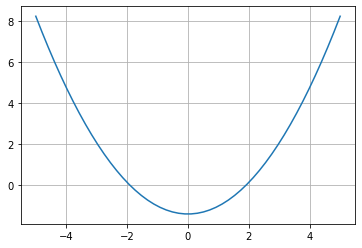
\includegraphics[scale=0.75]{images/2023-02-22-quadr_con_01.png}
\end{figure}

The next idea is that of partnering numbers; i.e. combining two numbers to simplify/enable calculations or proofs. Simple example is the sum of the first $49$ integers, $1 + 2 + \cdots + 49$. We partner two integers $x, y$ such that $x + y = 50$. This is shown in the following Figure.

\begin{figure}[H]
    \centering
    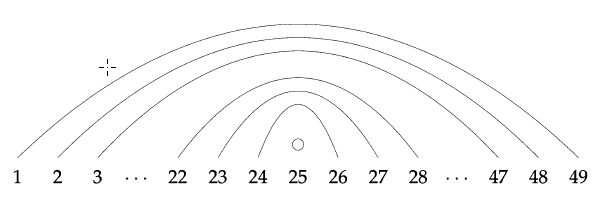
\includegraphics[scale=0.75]{images/2023-02-22-quadr_con_02.png}
\end{figure}

We have $24$ such pairs (which sum to $50$) and one left-over, which is $25$. We therefore can rewrite the sum as

\bee
1 + 2 + \cdots + 49 = 24 \times 50 + 25 = 1225 \qed
\eee

We use partnering to provide an additional proof to Wilson's theorem: I $p$ is prime, then

\bee
(p-1)! \equiv  -1 \mod p
\eee

In the product $(p-1)!$ we partner the numbers $(x,y)$ according to $x y \equiv 1 \mod p$; i.e. partner each number with its multiplicative inverse modulo-$p$. Since $p$ is prime, the inverse is unique and if a number has a partner, it is unique. The only numbers without a partner are those numbers $x$ which multiplicative inverse equals $x$ and these are $x = 1, p-1$.

So we have the $p-3$ numbers $2, 3, \cdots, p-2$ which can be paired according to $x y \equiv 1 \mod p$ and two left-overs $1$ and $p-1$. Multiplying all numbers together yields

\bee
(p-1)! = 2, 3, \cdots, p-2 \times 1 \times (p-1) \equiv 1 (p-1) \equiv (p-1) \equiv -1 \mod p
\eee

The following Figure shows these pairings for $p=13$: The numbers $2$ and $7$ are partners as $2 \cdot 7 \equiv 1 \mod 13$ as are $4$ and $10$, $4 \cdot 10 \equiv 1 \mod 13$. The only left-overs are $1$ and $12$ which are their own inverse. \qed

\begin{figure}[H]
    \centering
    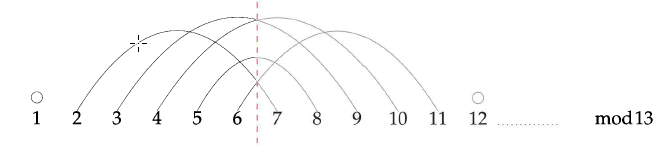
\includegraphics[scale=0.75]{images/2023-02-22-quadr_con_03.png}
\end{figure}

We can use this partnering concept to count the number of quadratic residues and nonresidues. The function $x^2 \mod p$ is a two-to-one correspondence; for every output there are exactely two inputs. As stated previouly, if $x$ and $p-x$ are input to the $x^2 \mod p$ function, they yield the same output, nnamely $x^2 \mod p$. On the other hand, no more than two inputs yield the same output. For if $x^2 \equiv y^2 \mod p$, we have $x^2-y^2\equiv 0 \mod p$ which can be factored as $(x-y)(x+y) \equiv 0 \mod p$ and we have $x \equiv  \pm y \mod p$. Since there are two inputs for each output, there are half as many outputs as inputs and therfore half of the numbners are quadratic residues.

The following Figure illustrates this for $p=11$. \qed

\begin{figure}[H]
    \centering
    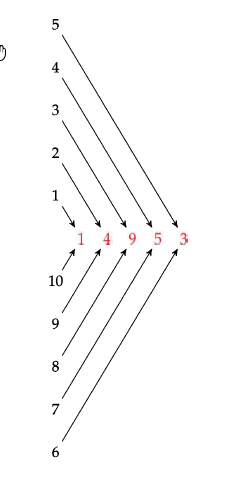
\includegraphics[scale=0.75]{images/2023-02-22-quadr_con_04.png}
\end{figure}

In the previous entry we covered Euler's Criterion for squareness: For an odd prime $p$ and $\gcd(a,p)=1$, $a$ is a quadratic residue of $p$ iff

\bee
a^{(p-1)/2} \equiv 1 \mod p
\eee

and a quadratic nonresidue iff

\bee
a^{(p-1)/2} \equiv -1 \mod p
\eee

This is actually a refinement of Fermat's Little Theorem which states that for a prime $p$ and $\gcd(a,p)=1$,

\bee
a^{p-1} \equiv 1 \mod p
\eee

Fermat's Little Theorem can be obtained from Euler's Criterion by squaring $a^{(p-1)/2} \equiv \pm 1 \mod p$. Thereby the sign information gets lost; in this sense, Fermat's Little Theorem is a weaker statement than Euler's Criterion. \qed




%%% Local Variables:
%%% mode: latex
%%% TeX-master: "journal"
%%% End:
